\documentclass{article}
\usepackage[font=small, labelfont=bf]{caption}
\usepackage{sectsty}
\usepackage{dblfloatfix} 
\usepackage{fixltx2e}
\usepackage{graphicx}
\usepackage{color}
\usepackage[letterpaper, margin=0.75in]{geometry}
\usepackage{amsmath}
\usepackage{amsfonts}
\usepackage{tikz}
\usepackage{pgfplots}
\usepackage{parskip}
\usepackage{multicol}
\usepackage{wrapfig}
\usepackage[compact]{titlesec}
\usepackage{float}
\usepackage{pdfpages}
\usepackage{euler}

\begin{document}
\graphicspath{ {Images/} }
\sectionfont{\fontsize{11}{0}\selectfont}
\setlength{\headsep}{0pt}

\titlespacing{\section}{0pt}{*0}{*0}
\titlespacing{\subsection}{0pt}{*0}{*0}
\titlespacing{\subsubsection}{0pt}{*0}{*0}

\setlength{\parindent}{0pt}

\title{Glycan Synthesis Through Staged Algorithmic Assembly}
\author{Anjali Jaiman and Mukund Thattai}
\maketitle


\section*{Supplemental:Reaction Network Definition}


Given that there is poor data about in vivo glycosyltransferase specificity and reaction ordering, it is difficult to useful glycan biosynthesis reaction network, especially post-code extensions. The reaction network can basically only be constructed through the assumed ordering of observed glycan products.

Typically the nodes of a reaction network are the set of measured molecular components of a reaction network, sometimes with extra nodes of presumed unobserved intermediates. For o-glycan biosynthesis such a reaction network would be a directed rooted acyclic graph. The set of internal nodes would include some unobserved intermediates (parisominous minimization of unobserved data suggests we choose a strict ordering of enzymes), and a parsimonious reaction network may have some observed products as internal nodes as well. All of the tips of the reaction network would be observed products. Such a reaction network assumes that there is high quality data of glycan products and attempts to minimize the number of unobserved structures in the model. The only biosynthetic insights such a reaction network can give easily give is understanding where high enzyme specificity (or mulitple enzymes) is required, implying that these are the central mechanisms by which limited heterogeneity is achieved. [Shall I put in a picture of a typical glycan reaction network?]

We use a different representation of the reaction network that gives more insight into potential mechanisms of control in glycan biosynthesis. We also use glycan data to construct the reaction network, but we assume that all enzymes are locally acting or post-node specific. The set of nodes represents the set of glycan monomers. An directed edge is placed between two nodes if these two nodes are seen in the data set as an acceptor-donor linkage pair, and the edge is labeled with the carbon number of the acceptor monosaccharide (because the donor linkage is usually 1 or 2). Such a reaction network is rooted and directed but may have cycles. The network will represent all observed reactions but will represent many [potentially infinitely many if there is a cycle] reaction intermediates. Such a reaction network is useful because it allows us to explore how reaction kinetics and compartmentalization may affect the set of observed and unobserved products.

\section*{Supplemental: Reaction Network Modeling}
In the following models we assumed that all enzymatic rates were equal. Since reactions are enzymatically driven, we assume all reverse reactions are neglible. We take all foward rates as 1. Thus all equations depend on a single parameter, the outshipping rate $\gamma$ (residence time $\frac{1}{\gamma}$). It should be noted, of course, that the assumption of a negible reverse reaction is not quite valid as the total residence time goes to infinity because the calculation then approaches an equilibrium system. It is true that a very different probability distribution on the glycan products might be found if the rates of different enzymatic steps are varied. However, we should state a few assumptions that make exploring these parameters unnecessary in our view. 

We assume a non-saturating condition, and thus all reaction rates can be considered independent of substrate concentration and we can set them all equal to unity. Thus the number of reactions are poisson distributed in time. The other stochastic event is the export from the reaction environment, which is drawn from an exponential distribution. Thus the only tunable parameter is the average amount of time each protein spends in the reaction environment. 

We can write down closed form solutions for the probability distributions on the set of final glycan products by solving the following:

\begin{equation} 
P(S,\beta,\gamma,c)=\int_0^\infty P(S,\beta,T)P(T,\gamma,c)dT
\end{equation}

Where $P(S,\beta,T)$ is the probability of building a particular structure in time, and $P(T,\gamma,c)$ is an exponential distribution if the number of compartments is 1 ($c=1$), but an erlang distribution for $c>1$. 

When the exit time distribution is no longer an exponential distribution, but a peaked distribution, the entropy of the distribution falls faster. This is obvious, but this is because the tails of the distribution are no longer large. What this implies is that for many peaked, small tailed waiting time distributions, the probability distribution tightens. Thus as we move away from a vesicle trafficking model, to a Golgi maturation model, in which the enzymes themselves move in retrograde vesicles. The compartment has a time dependent identity, with a peaked identity. This is like a peaked waiting time distribution, which will in many cases lead to a tigher probability distribution. 

\begin{enumerate}
\item We assume that the cell is noisy, but except for possibly structural glycans (which may require unlimited polymerization), the cell does aim to synthesize a particular set of glycan structures.
\item We assume that in an ordered reaction network these ``desired" products are saturated terminal species or nearly saturated species. If the were not desired in high abundances, the terminal enzymatic steps should not be expressed in the cell. 
\item In the long residence time limit, thus variable kinetics do not matter, because the residence time should be long enough to complete the terminal steps. 
\item Similarly in intermediate residence times, terminal reactions should not be so slow as to remain uncompleted (otherwise terminal products will not be formed).  
\end{enumerate}


\begin{figure}[h]
    \includegraphics[width=0.5\textwidth]{Figure_5.pdf}
	\caption{A)Entropy as a function of residence time comparing a cyclic reaction network, a cyclic reaction network with a competing tip and a totally ordered reaction network. B) Entropy as a function of residence time comparting a totally ordered reaction network. A partially ordered reaction network, and totally ordered reaction network with competition.}
\end{figure}

We are assuming that saturated, or almost saturated products are desired by the cell in high abundances (and possibly intermediates). If these terminal species were not   All analytical calculations were checked with gillespie simulations. Should I insert the figures here?

\section*{Supplemental: Totally Ordered Reaction Network}

For a totally ordered reaction network with L reactions, the probability of a structure with l<L of those reactions is:

\begin{equation} 
P(l,\beta,\gamma,c)=\int_0^\infty \frac{\gamma^ct^{c-1}}{(c-1)!}e^{-\gamma t}\frac{(\beta t)^l}{l!}e^{-\beta t})
\end{equation}

For a structure with l=L reactions and c compartments

\begin{equation}
P(L,\beta,\gamma,c)=\int_0^\infty \frac{\gamma^ct^{c-1}}{(c-1)!}e^{-\gamma t}(1-\sum_{n=0}^{L-1}\frac{(\beta t)^n}{n!}e^{-\beta t})
\end{equation}

Taking $\beta = 1$
\begin{equation}
P(l<L,\gamma,c)=\frac{(l+c-1)!}{l!(c-1)!}(\frac{1}{1+\gamma})^l(\frac{\gamma}{1+\gamma})^c
\end{equation}

\begin{equation}
P(L,\gamma,c)=1-\sum_{n=1}^{L-1}(\frac{(n+c-1)!}{n!(c-1)!}(\frac{1}{1+\gamma})^n(\frac{\gamma}{1+\gamma})^c)
\end{equation}

Since there is one terminal structure as $\tau \rightarrow\infty$, the entropy will go to zero. 

\section*{Supplemental: Competition in Reaction Network}
Competition comes from the colocalization of two or more enzymes that recognize the same substrate but are mutually exclusive in their action. A simple example is when two local enzmyes compete for the same carbon on the same acceptor monosaccharide. However, there are other kinds of competition. For example, if two enzymes have specificities that exclude the products of each other, although they could both act on the undecorated substrate. One enzyme might exclude the product of another, although the reverse might not be true. 

In our analytical calculation, we consider a reaction network with competition at site b at in a totally ordered reaction network, although we say that the subsequent reactions are identical. In this case, clearly the probabilities following the competitive reactions are just divided by 2. Note that this kind of competition does not terminate extension. 

\begin{equation}
P(l<b,\gamma,c)=\frac{(l+c-1)!}{l!(c-1)!}(\frac{1}{1+\gamma})^l(\frac{\gamma}{1+\gamma})^c
\end{equation}

\begin{equation}
P(b<=l<L,\gamma,c)=\frac{1}{2}\frac{(l+c-1)!}{l!(c-1)!}(\frac{1}{1+\gamma})^l(\frac{\gamma}{1+\gamma})^c
\end{equation}

\begin{equation}
P(L,\gamma,c)=\frac{1}{2}(1-\sum_{n=1}^{L-1}(\frac{(n+c-1)!}{n!(c-1)!}(\frac{1}{1+\gamma})^n(\frac{\gamma}{1+\gamma})^c))
\end{equation}


Since there are two competing terminal structures, as $\tau \rightarrow\infty$, the entropy will go to one (base 2). As long as the competitive events do not have different subsequent reaction topologies.  The number of terminal species will be $T=\prod_{i=1}^N (c_i)$, where $c_i$ is the number of competitive events at the ith site of competition. Each of these will have an equal probability (given the above stated symmetry of the reaction network), and entropy will be $\log_2(T)$. Note that in real reaction networks, what occurs after from a competitive event does is not symmetric, and therefore, the probability of finding two species that have different attachments at the same sites will not, in general be equal---even as  $\tau \rightarrow\infty$.


\section*{Supplemental: Partial Order in Reaction Network}

For a reaction network with two branches at the "zero" site, with lengths L1, and L2, but all reactions in the network have the same	 rates.

\begin{equation}
P(l1<L1,l2<L2,\gamma,c)=\frac{(l1+l2+c-1)!}{(c-1)!l1!l2!}(\frac{1}{2+c\gamma})^{l1+l2}(\frac{c\gamma}{2+c\gamma})^c
\end{equation}

\begin{equation}
P(l1<L1,L2,\gamma,c)=\frac{(l1+c-1)!}{(c-1)!l1!}(\frac{c\gamma}{c\gamma+1})^{l1+c}-\sum_{l2=0}^{L2-1}(\frac{l1+l2+c-1)!}{(c-1)!l1!l2!}\frac{(c\gamma)^c}{(c\gamma+2)^{l1+l2+c}}
\end{equation}

\begin{equation}
P(L1,L2,\gamma,c)=1-\sum_{l2=0}^{L2-1}(\sum_{l1=L1}^{L1-1}(P(l1<L1,l2<L2,\gamma,c)-\sum_{l1=0}^{L1-1}P(l1<L1,L2,\gamma,c)-\sum_{l2=0}^{L2-1}P(l2<L2,L1,\gamma,c)
\end{equation}


The number of intermediates in a partially ordered reaction network depends on at what depend of a tree branching occurs, and if a branch can be further extended or acts as a tip. 


To construct a partial order not at the root, but somewhere along the branch, we can just take the yield of a total ordered reaction network before the branch, 



\begin{equation}
P(l<B,\gamma,c)=\frac{(l+c-1)!}{l!(c-1)!}(\frac{1}{1+\gamma})^l(\frac{\gamma}{1+\gamma})^c
\end{equation}

\begin{equation}
P(l=B-1, l1<L1,l2<L2,\gamma,c)=P(l=B-1,\gamma,c)*P(l1<L1,l2<L2,\gamma,c)
\end{equation}

\begin{equation}
P(l=B-1, l1<L1,L2,\gamma,c)=P(l=B-1,\gamma,c)*P(l1<L1,L2,\gamma,c)
\end{equation}

\begin{equation}
P(l=B-1, l1<L1,L2,\gamma,c)=P(l=B-1,\gamma,c)*P(l1<L1,L2,\gamma,c)
\end{equation}


\section*{Supplemental: Tip Adding}
For a reaction network with polymerization and a competitive tip adder.

\begin{equation}
P(l=0)=\frac{\gamma}{1+\gamma}
\end{equation}

A chain of length $0<l$ with no cap
\begin{equation}
P(l, c=0,\gamma)=(\frac{1}{1+\gamma})^l\frac{1}{2^{l-1}}*(\frac{\gamma}{1+\gamma})
\end{equation}

A chain of length $1<l$ with a cap
\begin{equation}
P(l, c=1,\gamma)=(\frac{1}{1+\gamma})^l\frac{1}{2^{l-1}}
\end{equation}


As $\tau \rightarrow\infty$, the distribution becomes,

\begin{equation}
P(l=0,\gamma\rightarrow 1)\rightarrow 0
\end{equation}

\begin{equation}
P(l, c=0, \gamma\rightarrow 1)\rightarrow 0
\end{equation}

\begin{equation}
P(l, c=1, \gamma\rightarrow 1) \rightarrow \frac{1}{2^{l-1}}
\end{equation}

The entropy
\begin{equation}
E(\gamma\rightarrow 1)\rightarrow 2
\end{equation}

The entropy of this distribution as a function of $p=\frac{1}{1+\gamma}$ turns out to be (when simplified)

\section*{Supplemental: Entropy}
Note that for all graphs, entropy as a function of gamma is defined as:
\begin{equation}
E(\gamma)=\sum_{P(s,\gamma)}P(s,\gamma)*\log_2(P(s,\gamma))
\end{equation}



\section*{Supplemental:Abundances}
For each species represented, we calculated the range of residence times during which the species was greater than $5\%$ of the total. $5\%$ was chosen as an arbitrary cutoff, which allowed us to visualize all the species in the totally ordered set [A]. 
 
\begin{figure}[H]
    \includegraphics[width=\textwidth]{Supp_1.pdf}
	\caption{A)}
\end{figure}

\section*{Supplemental:Probability Distributions}
Here
\begin{figure}[H]
    \includegraphics[width=\textwidth]{Supp_2.pdf}
	\caption{A)}
\end{figure}

\begin{figure}[H]
    \includegraphics[width=\textwidth]{Supp_3.pdf}
	\caption{A)}
\end{figure}

\begin{figure}[H]
    \includegraphics[width=\textwidth]{Supp_4.pdf}
	\caption{A)}
\end{figure}

\section*{Supplemental}
\begin{figure}[H]
    \includegraphics[width=\textwidth]{Supp_5.pdf}
	\caption{A)}
\end{figure}

\section*{Supplemental: Compartmental Model}
Another reaction network representation was used to construct compartmentalized reaction network. First the dataset is decomposed into a set of unique links. A link is represented by an acceptor monosaccharide, donor monosaccharide and carbon linkage $E(A,D,C)$. If on any structure in the dataset $E1(A1,D1,C1)<E2(A2,D2,C2)$, linkage two occurs after linkage one, a directed edge from E1 to E2 is drawn. This reaction network represents a partially ordered set of locally acting enzymes ($E(A,D,C)$). Such a graph implies that enzyme one can act after enzyme two. There is an additional competition list stored. These are sets of enzymes that compete for the same acceptor monosaccharide and carbon linkage. $E1(A1,D1,C1)$and $E2(A2,D2,C2)$ compete if $A1=A2$, $C1=C2$ and $D1\neq D2$.


First we construct all maximal rooted acyclic subgraphs of the reaction network. 
\begin{enumerate}
\item All cycles in the reaction network stored as a set (ex Floyd's cycle-finding algorithm/Brent's cycle finding algorithm).
\item For each cycle of length $l_c$, all $l_c-1$ paths are stored as set A. 
\item All possible subsets of A are taken, and those with cycles are disgarded. This is the set of maximal acyclic subgraphs ($\left\{M_A\right\}$) of the cyclic components of reaction network R.
\item An additional ``common" rooted reaction network is constructed. This is the rooted component of the reaction network minus all enzymes involved in cycles ($R - \cup \left\{ M_A \right\}$). This is a single rooted acyclic graph (c). 
\item For each $a\in M_A$, we check if $a\cup c$ is connected. All such graphs are potential first compartment halting sets of enzymes, and we store each such graph along with it's corresponding ``interrupted cycles" $(h,a)\in H$. We also include $(c,0)\in H$.
\end{enumerate}

Note that when applied to dataset 1, the above step was unnecessary because the  maximal rooted acyclic subgraphs of the reaction network were easily constructed by hand. INSERT FIGURE. 

Next we developed a generative algorithm for constructing all non-polymerizing n-compartment ``partitions" from the reaction network. This algorithm attempted to minimize, but does not eliminate redundancy. And also note that this scheme gives many compartmentalization schemes that do not have all of the original enzymes represented in the original reaction network R. 

\begin{enumerate}
	\item Construct maximal halting k-compartments, by taking all possible orders of k elements of H (allowing reuse). These are compartmentalization schemes that allow maximal subgraphs of R elements without polymerization.
	\item For any single maximal halting k-compartmentalization scheme $[(h_1,a_1),(h_2,a_2)...(h_k,a_k)]$, we construct all possible first compartments (F) as follows.
\begin{enumerate}
	\item We generate all possible rooted subtrees of h, $\left\{s_{h1}\right\}$. 
	\item If  $s_{h1}\cap a \neq \emptyset$, then $(s_{h1},a,s_{h1}\cap c)\in F$ This simply reduces first compartment redundancy at the root of the tree.
\end{enumerate} 
\item We construct all possible second compartments for an first compartment $s_{h1}$ as follows:
\begin{enumerate}
\item  From the adjacency matrix eliminate all links s.t. $f\in c$ 
\item 
\end{enumerate} 
\end{enumerate}

To speed up the generative algorithm, some other things were done to enzyme that redundant graphs were not produced.

\section*{Supplemental: Constructing Glycans from Reaction Network}
Our encoding of glycan structures is a lexographical ordering of all paths root-->tip and root-->potential tip. 

\section*{Supplemental: Gillespie Simulation of Reaction Network}
A Gillespie simulation was designed to get the probability distribution over the set of structures in order to compare a one compartment model entropy with multiple compartment entropy. We took the set of unique local connections (acceptor monosaccharide, donor monosaccharide and carbon linkage) as the reaction set, and created a reaction network. All reactions were assumed to have the same reaction rates ($\beta=1$). The input substrate was assumed to be empty, and a single rooting reaction was first in the reaction network. At each step in the simulation the set of available acceptor monosaccharides was generated, and the set of enzymes that could act was generated. A random enzyme was selected from the acting set. Two waiting times were selected from the exponential distribution (one with rate $\beta = 1$, the other with rate $\gamma$). If the enzymatic reaction was selected, a random monomer was selected from the set of potential acceptor monosaccharides on the glycan. If export was selected, the glycan product was labeled "finished."

For a single compartment model all the reactions from dataset 1 were competed against eachother. For the multiple compartmental model, one of the "best 3-compartment model" described in Supplemental.... was selected. When the glycan was exported from the first compartment, it was passed as the input substrate into the second compartment. 

We consider enzyme catalyzed assembly with time dependent removal from the system; thus our set of final structures is determined by the algorithmic partition of the reaction network into compartments and by the 'fixing' of structures once they exit the synthesis environment. Reactions are driven by consumption of charged nucleotide-sugars; thus the system is not an equilibrium system, but we do not not what kind of non-equilibrium system it is. 

\section*{Supplemental: Enzyme Specificties}



\section*{Supplemental: Probability Distributions}
An array of average residence times (1/$\gamma$) were sampled: [0.1:1.5:97.8]. For each residence time, the simulation was run 10,000 times, and the entropy calculated. For the probability distribution graphs a list of all structures across all simulations was collected (1084 structures in total) and ordered according to the number of monomers in each structure. For each (procedure, residence time) an abundance vector of length 1084 was constructed. Any structure that had probability of less than 0.001 across all procedures was discarded (for a total of 74 structures). The x-axis of the probability distributions represents the number of monomers is the structure, and different structures with the same number of monomers are off-set. All structures above size 19 had probabilities of less than 0.001. The probabilities of these structures of size greater than 19 were summed and positioned at 20 on the x-axis. 


\section*{Supplemental: Additional Examples}
We recognize that these structures may not come from the same Golgi apparatus at all, and instead there are easy ways of constructing these four structures in higher abundance with three or four different programs. This would be a more traditional self-assembly approach whereby each structure is the desired output of a single program. For one structure two compartments is still required in order to prevent polymerization, but all other structures could be syntehsized as the terminating species of a single compartment. 

\section*{Supplemental:KL Divergences}
\begin{figure}[h]
    \includegraphics[width=\textwidth]{Figure_5.pdf}
	\caption{A)Entropy as a function of residence time comparing a cyclic reaction network, a cyclic reaction network with a competing tip and a totally ordered reaction network. B) Entropy as a function of residence time comparting a totally ordered reaction network. A partially ordered reaction network, and totally ordered reaction network with competition.}
\end{figure}



\section*{Supplemental Figure 1}

\section*{Supplemental Figure 2}

\begin{figure}[h]
    \includegraphics[width=\textwidth]{Supp_8.pdf}
	\caption{A)Entropy as a function of residence time comparing a cyclic reaction network, a cyclic reaction network with a competing tip and a totally ordered reaction network. B) Entropy as a function of residence time comparting a totally ordered reaction network. A partially ordered reaction network, and totally ordered reaction network with competition.}
\end{figure}


\section*{Supplemental Figure 3}

\section*{Supplemental Figure 4}
\end{document}


